\subsection{The functor TS}

Let M, N be A-modules and u a homomorphism of M into N; it is clear that \(\mathbf{T}(u)(\mathbf{TS}(\mathbf{M})) \subset \mathbf{TS}(\mathbf{N})\) . The mapping of \(\mathbf{TS}(\mathbf{M})\) into \(\mathbf{TS}(\mathbf{N})\) obtained from \(\mathbf{T}(u)\) is denoted by \(\mathbf{TS}(u)\) . It is easily verified that this is a unital homomorphism of graded algebras and we have \(\mathbf{TS}(u)\left(\gamma_{p}(x)\right) = \gamma_{p}(u(x))\) for all \(x \in M\) and each integer \(p \geqslant 0\) . If \(v : N \to P\) is a homomorphism of A-modules, we have

\[
\mathbf {T S} (v \circ u) = \mathbf {T S} (v) \circ \mathbf {T S} (u).
\]

By definition of TS(u), the diagram

\pandocbounded{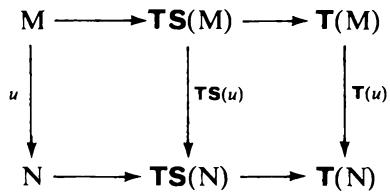
\includegraphics[keepaspectratio]{images/part001_53632150.jpg}}

is commutative, where the horizontal arrows denote canonical injections.

If M is a direct factor of N and \(i: M \rightarrow N\) is the canonical injection, then \(\mathbf{TS}(i)\) is an injective homomorphism of \(\mathbf{TS}(\mathbf{M})\) onto a direct factor R of \(\mathbf{TS}(\mathbf{N})\) , by which we normally identify \(\mathbf{TS}(\mathbf{M})\) and R. That is proved as for the tensor algebra (III, p.~487).

Suppose that M is a direct sum of a family \((\mathbf{M}_{\lambda})_{\lambda \in L}\) of submodules. The canonical injections \(\mathbf{TS}(\mathbf{M}_{\lambda}) \to \mathbf{TS}(\mathbf{M})\) define a unital homomorphism h of graded algebras, called canonical:

\[
\underset {\lambda \in L} {\otimes} \mathbf {T S} \left(\mathrm{M} _ {\lambda}\right)\rightarrow \mathbf {T S} (\mathrm{M}).
\]

Let \(\lambda_1, \lambda_2, \ldots, \lambda_n\) be pairwise distinct elements of \(L\) and let \(x_1 \in M_{\lambda_1}, \ldots, x_n \in M_{\lambda_n}\) . By Prop. 3, (ii) of IV, p.~45 we have

\[
h \left(\sum_ {p _ {1} + \dots + p _ {n} = p} \gamma_ {p _ {1}} (x _ {1}) \otimes \dots \otimes \gamma_ {p _ {n}} (x _ {n})\right) = \gamma_ {p} (x _ {1} + \dots + x _ {n}).\tag{8}
\]

Let N be an A-module which is a direct sum of a family \((\mathbf{N}_{\lambda})_{\lambda \in L}\) of submodules. For every \(\lambda \in L\) let \(u_{\lambda}\) be a homomorphism of \(M_{\lambda}\) into \(N_{\lambda}\) . Let u be the homomorphism of M into N defined by the \(u_{\lambda}\) . Then the diagram

\[
\begin{array}{c} \otimes \mathsf {T S} (\mathrm{M} _ {\lambda}) \xrightarrow {h} \mathsf {T S} (\mathrm{M}) \\ \otimes \mathsf {T S} (u _ {\lambda}) \Bigg | _ {\downarrow} \qquad \qquad \qquad \qquad \qquad \qquad \qquad \qquad \qquad \qquad \qquad \qquad \qquad \qquad \qquad \qquad \qquad \qquad \qquad \qquad \qquad \qquad \qquad \qquad \qquad \qquad \qquad \qquad \qquad \qquad \qquad \qquad \qquad \qquad \\ \otimes \mathsf {T S} (\mathrm{N} _ {\lambda}) \xrightarrow {h ^ {\prime}} \mathsf {T S} (\mathrm{N}) \end{array}
\]

commutes, where h and \(h'\) are canonical homomorphisms. For if \(z \in TS(M_{\lambda})\) and if \(i_{\lambda}\) (resp. \(j_{\lambda}\) ) denotes the canonical injection of \(M_{\lambda}\) into M (resp. \(N_{\lambda}\) into N), then we have

\[
\begin{array}{r l} \mathbf {T S} (u) (h (z)) & = \mathbf {T S} (u) \circ \mathbf {T S} (i _ {\lambda}) (z) = \mathbf {T S} (u \circ i _ {\lambda}) (z) = \\ & = \mathbf {T S} (j _ {\lambda} \circ u _ {\lambda}) (z) = \mathbf {T S} (j _ {\lambda}) \circ \mathbf {T S} (u _ {\lambda}) (z) = h ^ {\prime} (\mathbf {T S} (u _ {\lambda}) (z)). \end{array}
\]

PROPOSITION 6. --- Let M be an A-module which is the direct sum of a family \((\mathbf{M}_{\lambda})_{\lambda \in L}\) of submodules. If each \(M_{\lambda}\) is a free module, then the canonical homomorphism of \(\otimes \mathbf{TS}(\mathbf{M}_{\lambda})\) into \(\mathbf{TS}(\mathbf{M})\) is an isomorphism.

Let \((e_{i,\lambda})_{i\in I_{\lambda}}\) be a basis of \(\mathbf{M}_{\lambda}\) . For \(\nu \in \mathbf{N}^{(I_{\lambda})}\) put \(e_{\nu ,\lambda} = \prod_{i\in I_{\lambda}}\gamma_{\nu (i)}(e_{i,\lambda})\) . The \(e_{\nu ,\lambda}\) for \(\nu \in \mathbf{N}^{(I_{\lambda})}\) form a basis of \(\mathbf{TS}(\mathbf{M}_{\lambda})\) (IV, p.~47, Prop. 4 (i)) and \(e_{0,\lambda}\) is the unit-element of \(\mathbf{TS}(\mathbf{M}_{\lambda})\) . Therefore the elements

\[
\bigotimes_ {\lambda \in L} e _ {\nu_ {\lambda}, \lambda}\tag{9}
\]

where \(\nu_{\lambda} \in \mathbf{N}^{(I_{\lambda})}\) and \(\nu_{\lambda} = 0\) except for a finite number of indices, form a basis of \(\otimes_{\lambda} \mathbf{TS}(M_{\lambda})\) . The image of the element (9) under the canonical homomorphism of the proposition is \(\prod_{\lambda \in L} e_{\nu_{\lambda,\lambda}}\) . If we denote by \((e_i)_{i \in I}\) the disjoint union of the families \((e_{i,\lambda})_{i \in I_{\lambda}}\) , then the above elements are precisely \(\prod_{i \in I} \gamma_{\nu(i)}(e_i)\) , where \(\nu \in \mathbf{N}^{(I)}\) , and so they constitute a basis of \(\mathbf{TS}(M)\) . This proves the proposition.

Under the conditions of Prop. 6, the inverse isomorphism \(\mathbf{TS}(\mathbf{M}) \to \otimes_{\lambda} \mathbf{TS}(\mathbf{M}_{\lambda})\) is also called canonical. Frequently \(\mathbf{TS}(\mathbf{M})\) is identified with

\(\otimes_{\lambda} \mathbf{TS}(M_{\lambda})\) by means of this isomorphism. It should be noted that if \(z \in \mathbf{TS}(M_{\lambda})\)

\pandocbounded{
\includegraphics[keepaspectratio]{images/part001_3a9079a2.jpg}}

and \(z' \in \mathbf{TS}(M_{\mu})\) with \(\lambda \neq \mu\) , then the element of TS(M) which we are thus led to denote by \(z \otimes z'\) is not the tensor product of z and \(z'\) in T(M) but the symmetric product of z and \(z'\) .

PROPOSITION 7. --- Let M be an A-module, u the mapping \((x, y) \mapsto x + y\) of \(M \oplus M\) into M and f the composite mapping

\[
\mathbf {T S} (\mathrm{M}) \otimes \mathbf {T S} (\mathrm{M}) \xrightarrow {h} \mathbf {T S} (\mathrm{M} \oplus \mathrm{M}) \xrightarrow {\mathbf {T S} (u)} \mathbf {T S} (\mathrm{M})
\]

where \(h\) is the canonical homomorphism. If \(z, z' \in \mathbf{TS}(\mathbf{M})\) , then \(f(z \otimes z') = zz'\) .

For let \(i\) be the mapping \(x \mapsto (x, 0)\) of M into M ⊕ M. We have \(u \circ i = \mathrm{Id}_{\mathbf{M}}\) , hence \(\mathbf{TS}(u) \circ \mathbf{TS}(i) = \mathrm{Id}_{\mathbf{TS}(\mathbf{M})}\) ; therefore

\[
f (z \otimes 1) = \mathbf {T S} (u) (h (z \otimes 1)) = \mathbf {T S} (u) (\mathbf {T S} (i) (z)) = z.
\]

Likewise \(f(1 \otimes z') = z'\) , whence \(f(z \otimes z') = f(z \otimes 1)\) \(f(1 \otimes z') = zz'\) .

